% Five experiments to settle the Pais patents -- open technical report (v1.0)
\documentclass[10.5pt,a4paper]{article}
\usepackage[a4paper,margin=2.2cm,top=2.0cm,bottom=2.2cm]{geometry}
\usepackage{amsmath}
\usepackage{fontspec}
\usepackage{unicode-math}
\setmainfont{DejaVu Sans}[Scale=0.88]
\setsansfont{DejaVu Sans}[Scale=0.88]
\setmonofont{DejaVu Sans Mono}[Scale=0.84]
\setmathfont{DejaVu Math TeX Gyre}[Scale=0.88]
\usepackage{graphicx}
\usepackage{booktabs,tabularx,array,colortbl}
\usepackage{xcolor}
\usepackage{enumitem}
\usepackage{microtype}
\usepackage{titlesec}
\usepackage{fancyhdr}
\usepackage{caption}
\usepackage{tcolorbox}
\usepackage{float}
\usepackage[colorlinks=true,linkcolor=blueacc,citecolor=blueacc,urlcolor=blueacc]{hyperref}
\newcommand{\AUTHOR}{Spheromax}


\definecolor{ink}{HTML}{0A1628}
\definecolor{slate}{HTML}{4A5B70}
\definecolor{accent}{HTML}{C8761E}
\definecolor{blueacc}{HTML}{2F5FA8}
\definecolor{greenacc}{HTML}{2E8B57}
\captionsetup{font=small,labelfont=bf}
\setlist{nosep,leftmargin=1.3em}
\titleformat{\section}{\normalsize\bfseries\color{ink}}{\color{accent}\thesection}{0.7em}{\MakeUppercase}
\titleformat{\subsection}{\normalsize\bfseries\color{blueacc}}{\thesubsection}{0.6em}{}
\titlespacing*{\section}{0pt}{1.2ex plus .4ex}{0.6ex}
\titlespacing*{\subsection}{0pt}{1.0ex plus .3ex}{0.4ex}
\pagestyle{fancy}\fancyhf{}
\renewcommand{\headrulewidth}{0pt}
\lfoot{\footnotesize\ttfamily\color{slate}SPHEROMAX\enspace$\cdot$\enspace Pais gap loop\enspace$\cdot$\enspace open report v1.0}\rfoot{\footnotesize\ttfamily\color{slate}\thepage}
\newcommand{\e}[1]{\times10^{#1}}
\newcommand{\un}[1]{\,\mathrm{#1}}
\newcommand{\Kc}{K$_3$C$_{60}$}
\hypersetup{pdftitle={Five Experiments to Settle What Is Left of the Pais Patents},pdfauthor={\AUTHOR},pdfsubject={Open designs, costs and the meaning of each result: final report of the Pais gap research loop},pdfkeywords={Pais patents; inertial mass reduction; REBCO; light-gas gun; free-electron laser; K3C60; torsion balance; propellantless propulsion; open hardware; ethical source}}

\newcommand{\testhead}[2]{\subsection*{#1\quad\textmd{\ttfamily\small\color{accent}#2}}}
\newcommand{\sep}{\texorpdfstring{\,\textperiodcentered\,}{ - }}
\newcommand{\lab}[1]{\par\smallskip\noindent\textbf{#1}\enspace}

\begin{document}

\begin{center}
{\LARGE\bfseries\color{ink} FIVE EXPERIMENTS TO SETTLE WHAT IS LEFT\\[3pt] OF THE PAIS PATENTS}\\[7pt]
{\ttfamily\color{slate} Open designs, costs and what each result would mean}\\[1pt]
{\ttfamily\color{slate} Final report of the Pais gap research loop}\\[10pt]
{\large\bfseries\color{ink} \AUTHOR}\\[3pt]
{\small\ttfamily\color{slate} version 1.0 $\cdot$ 14 November 2026 $\cdot$ open technical report}
\end{center}

\begin{tcolorbox}[colback=white,colframe=accent,coltitle=white,boxrule=0.7pt,arc=1.5pt,left=8pt,right=8pt,top=6pt,bottom=6pt,title={\small\bfseries PURPOSE AND LICENCE}]
\small
\emph{This work is for humanity. It may not be used for war, for greed, or for any inhumane purpose. It is offered so that people can become more humane, and for our advancement in technology and in spirit, in harmony and balance.}\par\smallskip
Everything in this record is released under the Hippocratic License 3.0 with the Military Activities module (HL3-MIL), \url{https://firstdonoharm.dev}. The one exception is the film's soundtrack, whose rights are reserved. You may use, study, build, test, share and improve it for peaceful and humane purposes. The author has filed no patent on this work; publishing it openly is meant to keep it free for everyone.
\end{tcolorbox}

\noindent{\ttfamily\bfseries\color{ink}THE RESULT\enspace}
An AI-assisted research loop examined, gap by gap, the physics claims in the US Navy patents of Salvatore Pais (an ``inertial mass reduction'' craft, a high-energy electromagnetic field generator, a high-frequency gravitational-wave generator, a plasma compression fusion device and a room-temperature superconductor) and related claims of propellantless thrust and light-driven superconductivity. Over eleven runs it logged 162 literature searches with sources, built a ledger of 36 settled results (first-principles derivations with independently recomputed numbers, and published measurements), and stopped by its own rule when further searching no longer changed the picture. Nothing in the patents survives as physics: their central flux formula is contradicted by everyday ultrasound transducers by a factor of about $10^{24}$, and stored field energy or spin can only raise inertial mass, by at most $2\e{-9}$ of the structure. What survives is engineering: a magnetically held rotor and a light-driven film kept on inside a laser cavity. Two further claims can only be settled by null tests. This report sets out five experiments that decide what is left, with concept designs, A3 drawings, CAD, rough costs (about \$4--9M in total, about \$1--2M for the first two answers) and what each outcome would mean.

\section{Why this work}
The Pais patents, granted or published in 2018 and 2019 \cite{p532,p366,p827,p733,p597}, describe devices that would change propulsion, energy and materials if they worked. They drew wide public attention, and the Naval Air Warfare Center tested the central effect from 2016 to 2019 for about \$0.5M without being able to demonstrate it (Supplement S1). Similar claims circulate alongside them: a charged-dielectric thruster said to give millinewtons in vacuum from microwatts (the ``X1'') \cite{exodus}, and a light-driven, superconducting-like state in the fulleride \Kc{} \cite{mitrano}.

This work asked, for each claim, what it would physically require, how far that is from what nature and materials allow, and which experiment would decide whatever is left. The answer is short: almost everything is already settled by known physics, and five experiments, most of them small, would settle the rest.

\section{How the work was done}
\textbf{The loop.} The work ran as a repeating research loop of three steps: (A) plan and search the literature, logging every search with its title and link; (B) derive the physics from first principles and compute every number in code; (C) score the run and rewrite the loop's state file, so that each run started from what the previous one had learned. Each claim was reduced to a \emph{gap}: the factor between what it needs and what has been achieved, and the wall (atoms, materials, the vacuum, engineering) that sets the limit.

\textbf{Checks.} Each run re-derived its key numbers with independent code (``canary'' checks), and passed a 14-signal health test with thresholds fixed in advance (repeated queries, recycled sources, topic concentration, exploration, novelty, progress, circularity and others). Errors that were caught are logged in the state file. Evidence is graded A (replicated), B (one peer-reviewed measurement), C (preprint or conference), D (theory or estimate) and E (claim).

\textbf{Stopping.} The loop's rule was to stop when every gap is settled, or when two runs in a row move nothing. After run 11 every gap was closed, against a wall, or reduced to deciding experiments; run 11 moved nothing and its novelty and progress signals turned red, so the loop stopped. In total: 11 runs, 162 logged searches, 36 ledger entries and a 40-page mathematics run sheet (Supplement S1).

\textbf{Use of AI.} This work was carried out by the author with Claude (Anthropic), a large language model, used as a research assistant. The author set the questions and goals, directed the loop and its side questions, chose which paths to keep, and asked for the test designs, drawings, film and this report. Claude ran and logged the literature searches, derived and computed the results (all code is included, Supplement S5), designed the concept rigs and drawings, and drafted the text. AI tools are not listed as authors. The author has reviewed this report and takes responsibility for its publication; readers should check any number against the code and sources before relying on it.

\section{What the loop settled}
Figure~\ref{fig:status} shows the final status of the eleven gaps and the five deciding tests. The main results are these.
\begin{itemize}
\item \textbf{The flux formula is not radiation.} Pais's flux formula reproduces his own numbers ($1.18\e{24}\un{W/m^2}$) but describes an energy density carried at a surface speed, not radiated power. A steadily spinning or uniformly breathing charged body radiates nothing.
\item \textbf{The formula is already falsified.} A capacitive ultrasound transducer is a charged plate at about $10^8\un{V/m}$ vibrating at megahertz: every ingredient of the patents' Eq.~2. Eq.~2 predicts about $8.7\e7\un{W}$ from each square centimetre of such a probe; known physics gives $10^{-16}\un{W}$; real probes run on a few watts.
\item \textbf{Fields and spin cannot reduce mass.} For any material-supported field or spinning body, the stored energy raises inertial mass, by at most about $2\e{-9}$ of the structure (a consequence of von Laue's theorem and the strength of materials). Electric charge leaves weight unchanged to $2\e{-3}$ in a direct test \cite{hathaway}.
\item \textbf{No self-push.} A closed system cannot push itself: thrust without propellant is at most $P/c = 3.34\un{nN}$ per watt. Independent balances have bounded EMDrive-type devices below that \cite{tajmar21}.
\item \textbf{The required fields exceed what atoms can hold.} The patents' surface charge ($5\e4\un{C/m^2}$) implies fields $10^4$ times the atomic field; surfaces field-evaporate long before. Their $10^6\un{T}$ is $10^3$ beyond the strongest field ever made with matter.
\end{itemize}
Two engineering paths survived. \textbf{B6} is a rotor held by a superconducting stator, so that the stator rather than the rim's own strength carries the load; it is limited by field quality, conductor temperature and containment, which three measurements decide (T1, T2). \textbf{B7} keeps a light-driven state in a thin \Kc{} film switched on by placing the film inside a free-electron-laser cavity, so the source only pays for what the film absorbs; one experiment decides it (T3). Two claims can only be closed by null tests: any coupling between electromagnetism and gravity (T4), and the X1 thrust (T5).

\begin{figure}[t]
\centering
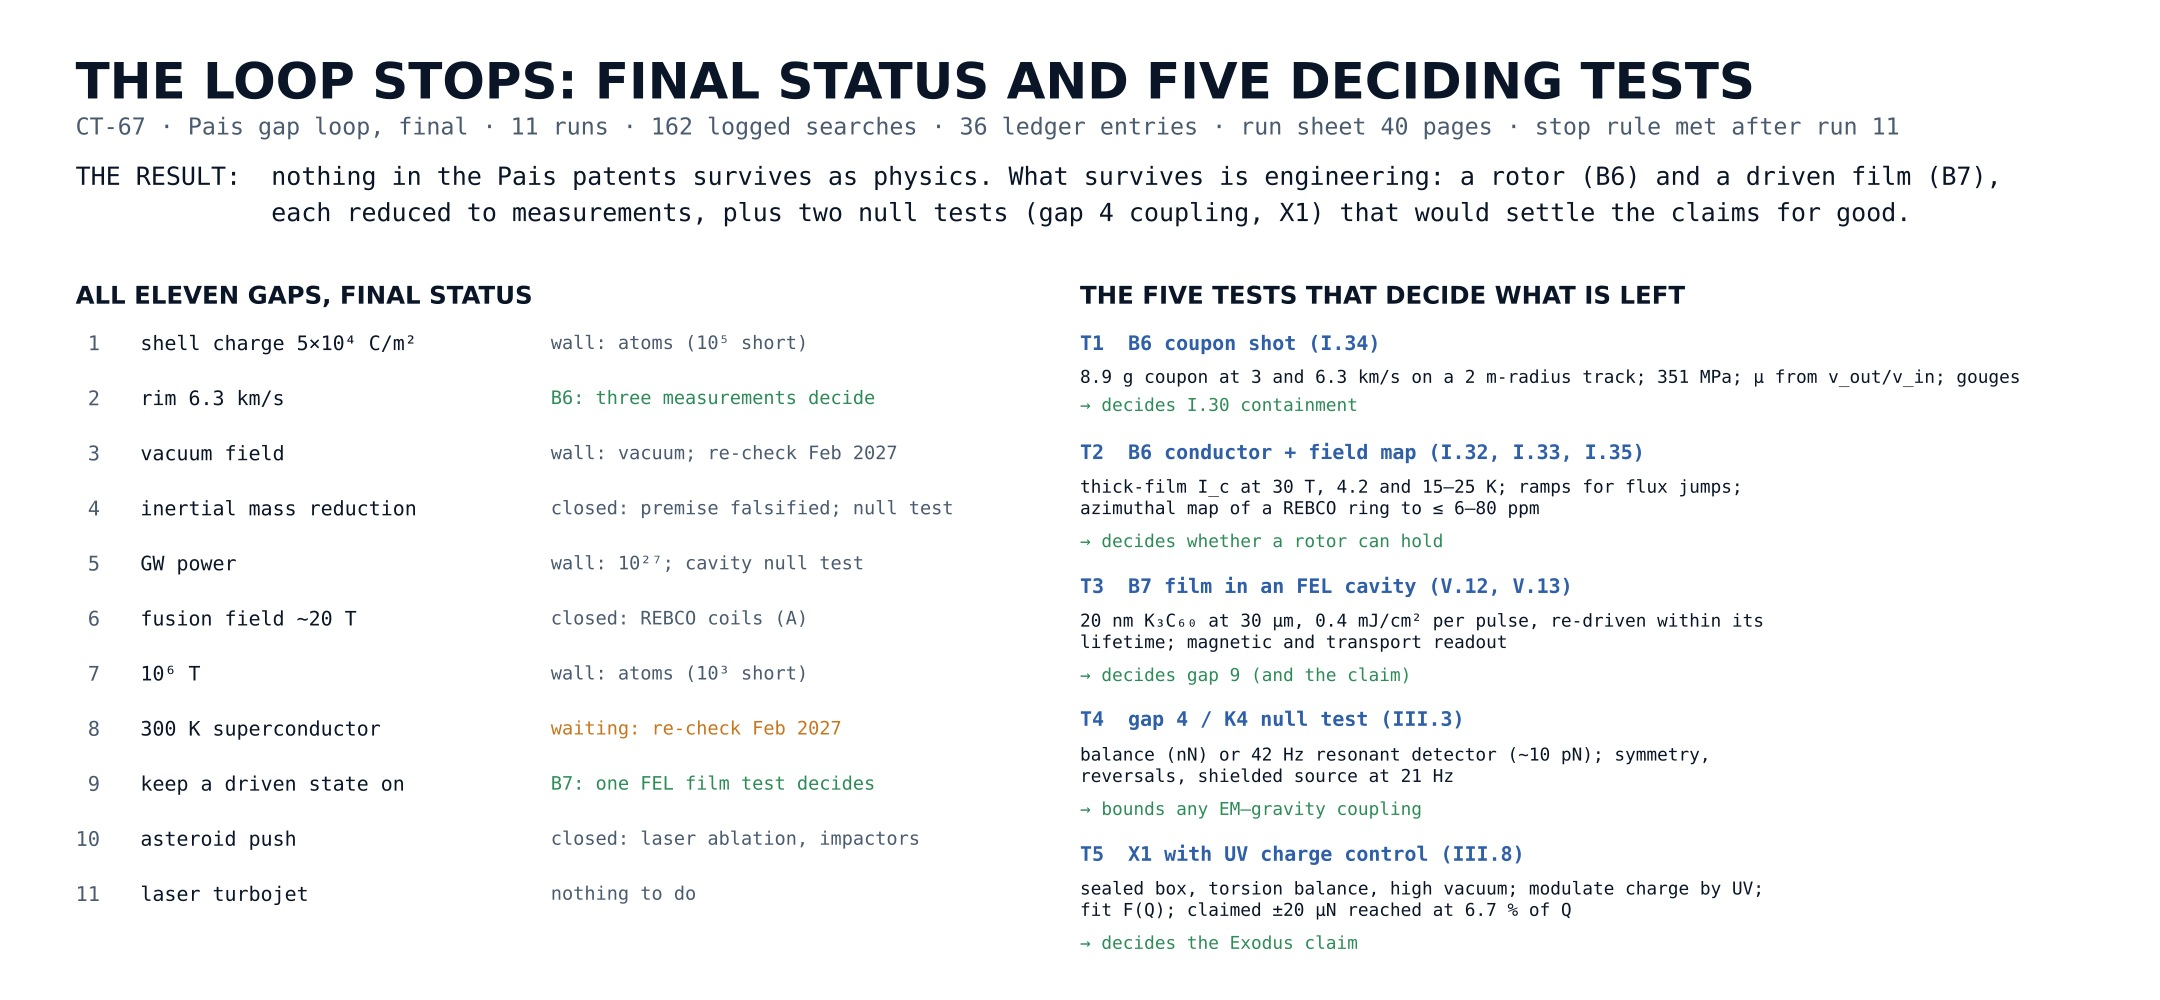
\includegraphics[width=\textwidth]{fig/ct67_top_light.jpg}
\caption{Final status of the eleven gaps (left) and the five tests that decide what is left (right), from the loop's last summary sheet. Item numbers (I.30, V.13, III.8, ...) refer to the mathematics run sheet (Supplement S1).}
\label{fig:status}
\end{figure}

\section{The five deciding tests}
The tests are listed in the recommended order: cheapest and fastest first. Concept designs, A3 drawings and CAD for every rig are in Supplements S2 and S3; the full derivations are in S1.

\testhead{T5\sep The X1 claim with UV charge control}{about \$0.2--0.5M}
\lab{What it decides.} Whether the X1 ``new force'' is ordinary electrostatics from trapped charge. The claimed 4.46\,mN at $228\,\mu$W is $5.7\e5$ times what ejected ions could give, and it equals the pull of $5.6\,\mu\mathrm{C/m^2}$ of trapped charge, which relaxes in minutes (polyimide) to days (PTFE).
\lab{Setup.} The thruster inside a sealed, grounded conducting box on a torsion balance in high vacuum. Its trapped charge is changed with 254\,nm UV LEDs (4.88\,eV, above the work function) or an electron flood, as in LISA Pathfinder's charge control; air ionizers do not work in vacuum.
\lab{Numbers.} Trapped charge $Q=1.41\e{-8}\un{C}$; force $F=cQ^2$ with $c=2.26\e{13}\un{N/C^2}$. Photocurrents of 1, 10 and 100\,nA discharge it in 14, 1.4 and 0.14\,s. At 30, 10 and 1\,\% of $Q$ the force is 401, 44.6 and $0.45\,\mu$N; the claimed $\pm20\,\mu$N resolution is reached at 6.7\,\% of $Q$.
\lab{Pass or fail.} Fit $F$ against $Q$. If $F\propto Q^2$ and goes to zero as the charge is removed, the force is electrostatic and the claim is closed. If a force stays with the charge removed, inside a sealed box, in vacuum, with reversals, it is anomalous and should go to outside laboratories for replication. The test needs an X1 device, from the claimants or built from their published filings \cite{exodus}.

\begin{figure}[H]
\centering
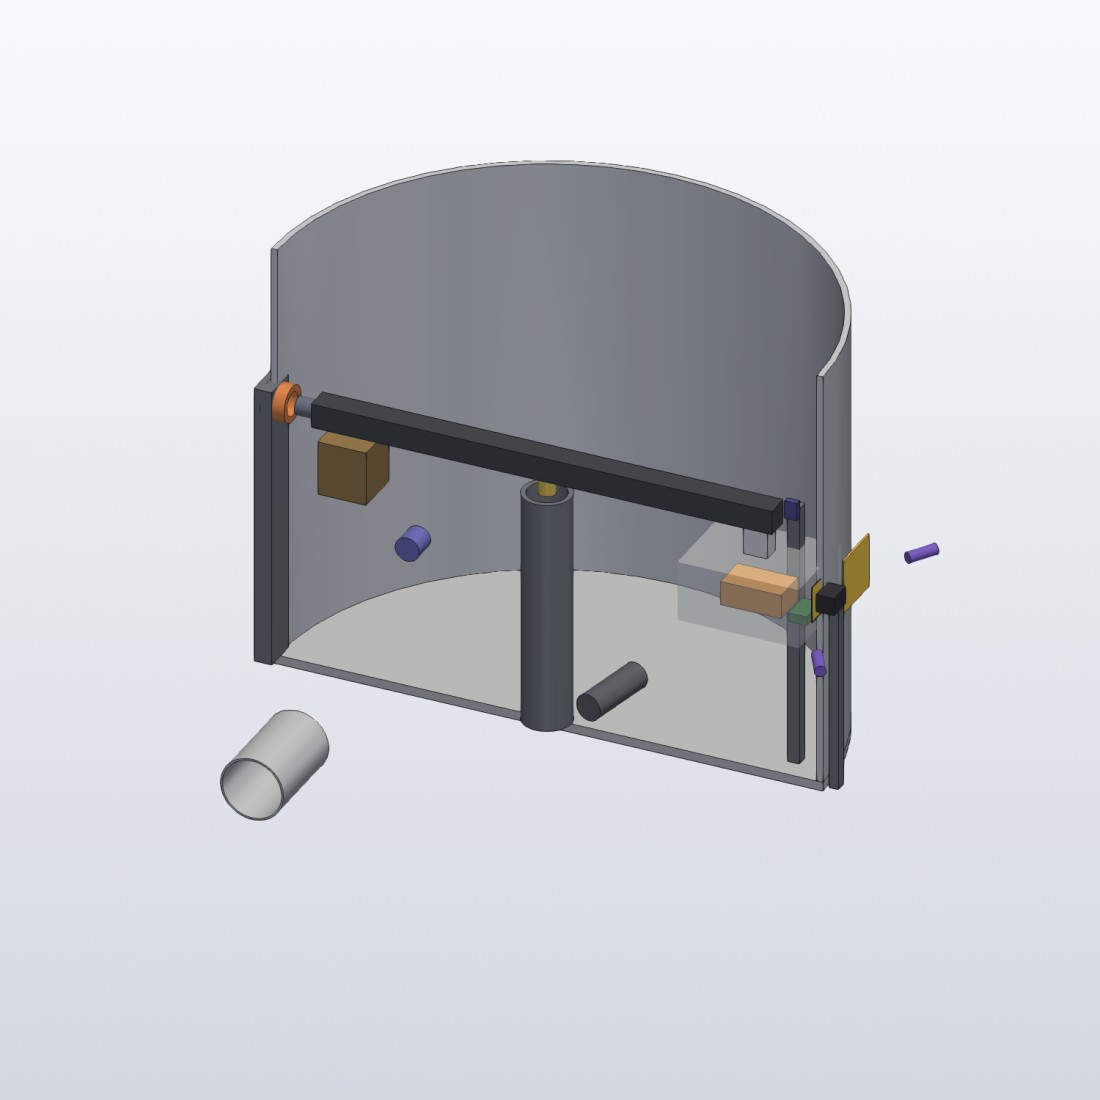
\includegraphics[width=0.36\textwidth]{fig/T5_balance_cutaway.jpg}\hspace{4mm}
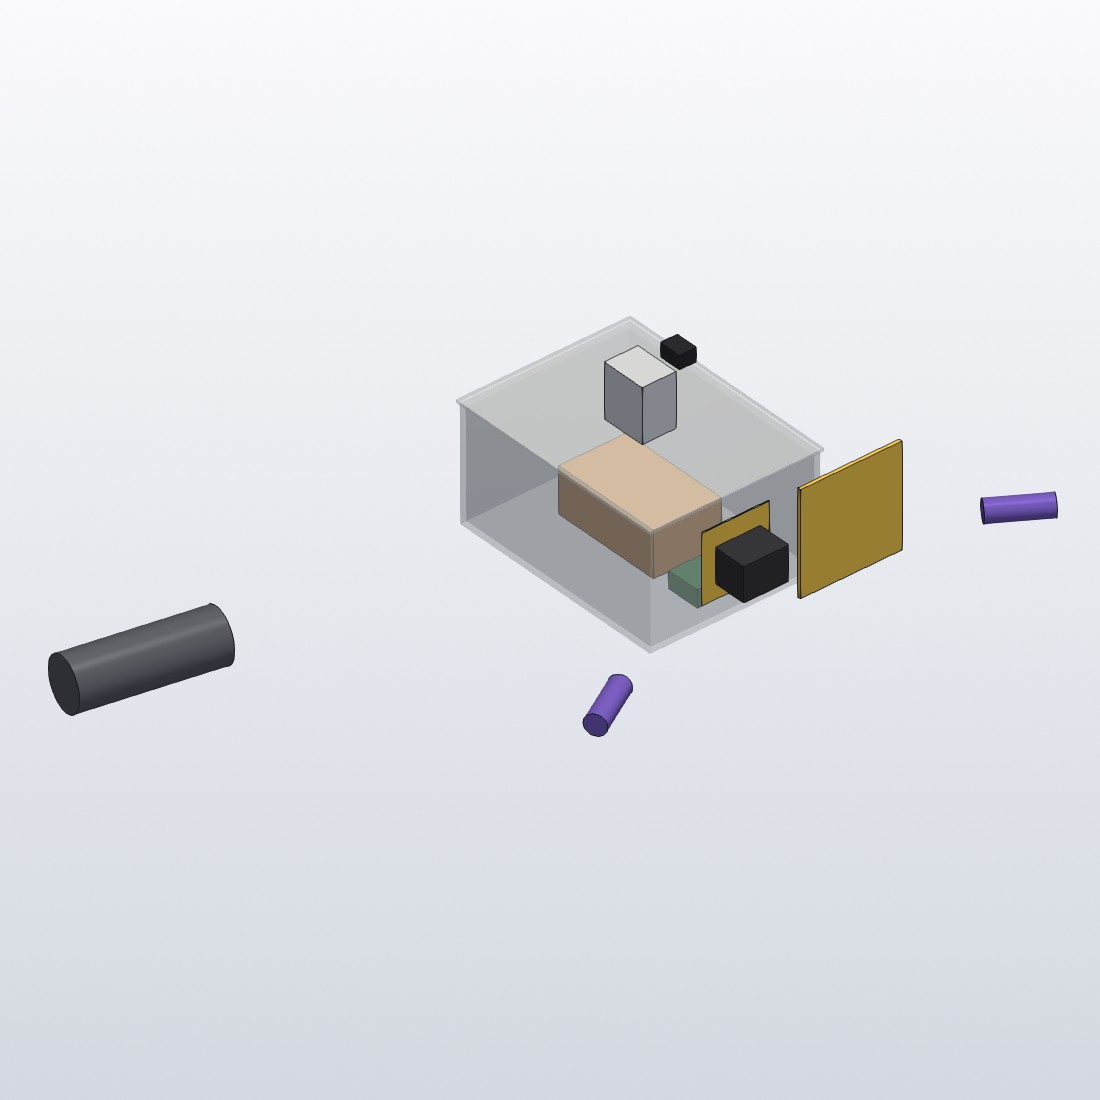
\includegraphics[width=0.30\textwidth]{fig/T5_box_iso.jpg}
\caption{T5 concept: torsion balance in a vacuum chamber (cutaway, left); the sealed, grounded box with UV LEDs and an electron flood gun (right).}
\end{figure}

\testhead{T4\sep Field--gravity null test}{about \$0.7--1.3M}
\lab{What it decides.} Whether electromagnetic fields couple to gravity or inertia beyond known physics: the premise of the ``inertial mass reduction'' patent. Known physics predicts nothing measurable: the field mass of a laboratory rig is $+5.2\e{-19}\un{kg}$ and its radiated thrust at most $3.7\e{-16}\un{N}$.
\lab{T4a: balance.} A shielded, battery-powered rig in high vacuum on a nN-class balance: a Pais-type charged disk (30\,cm, $1\,\mu$C, 94\,kV, vibrated $\pm80$\,nm at 100\,MHz) or a capacitor and coil set. Protocol: face-to-face symmetry better than $2\e{-6}$ (the image pressure pulls 0.050\,N per face), polarity reversal, the device rotated $180^\circ$ in vacuum, then discharged, spin-only and vibration-only runs. TU Dresden found no coupling at about 1\,nN with steady fields \cite{tajmar24}; high-frequency fields are the open edge.
\lab{T4b: resonant detector.} ETH Z\"urich's 42\,Hz bending-beam detector ($Q\approx10^4$, picometre readout) measured dynamic gravity to about 3\,\% of theory \cite{brack22}. With a shielded electromagnetic source whose field energy oscillates at 42\,Hz (driven at 21\,Hz) in place of the moving mass, it resolves roughly 7--28\,pN, 36--140 times below a nN balance.
\lab{Pass or fail.} Any reproducible signal that survives reversal, rotation and shielding, and exceeds the computed Newtonian and electromagnetic crosstalk, is new physics. A null bounds any coupling at the instrument's floor and closes the premise experimentally, as it is already closed in theory.

\begin{figure}[H]
\centering
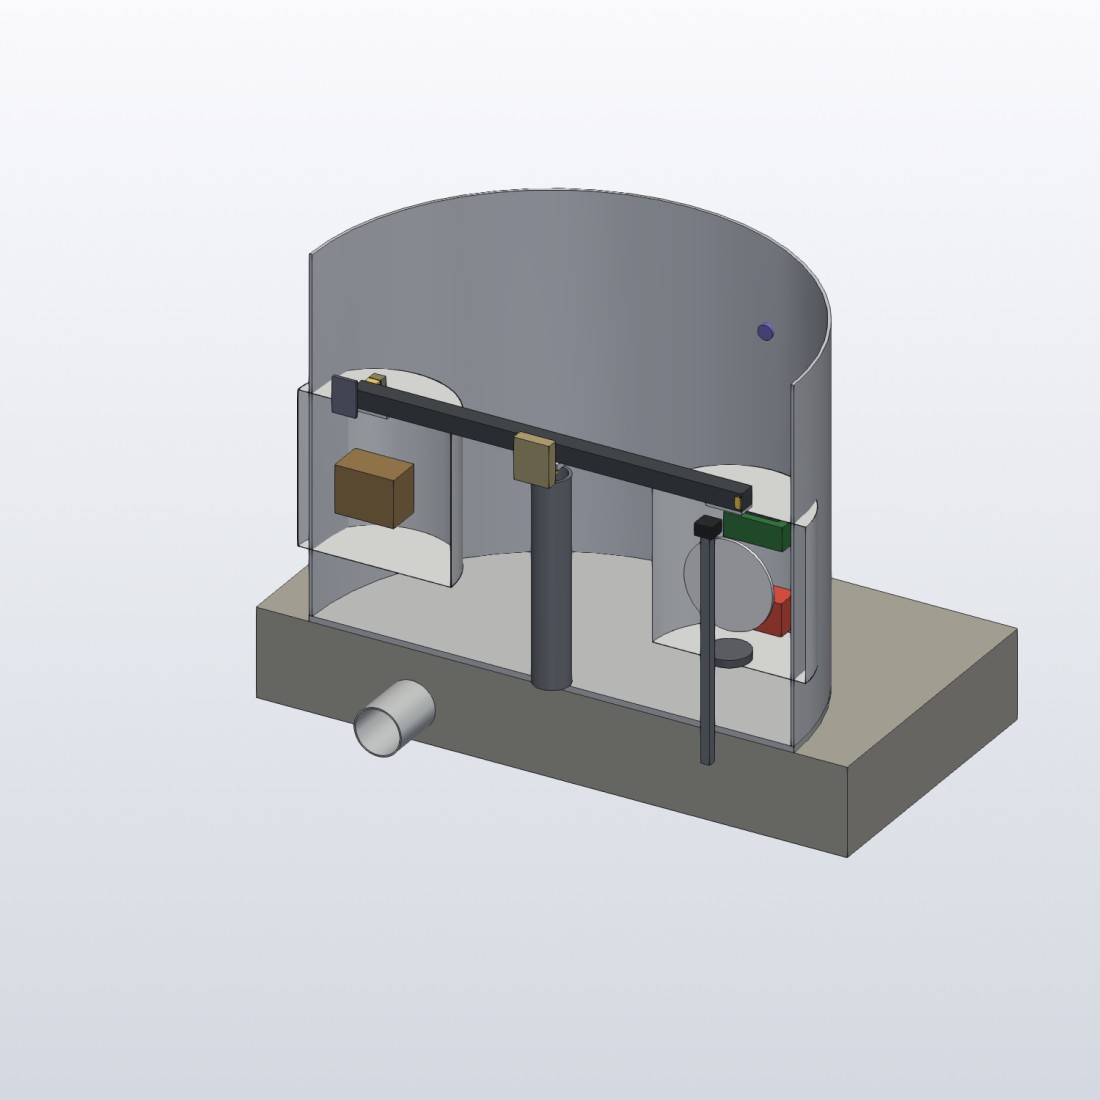
\includegraphics[width=0.34\textwidth]{fig/T4a_balance_cutaway.jpg}\hspace{4mm}
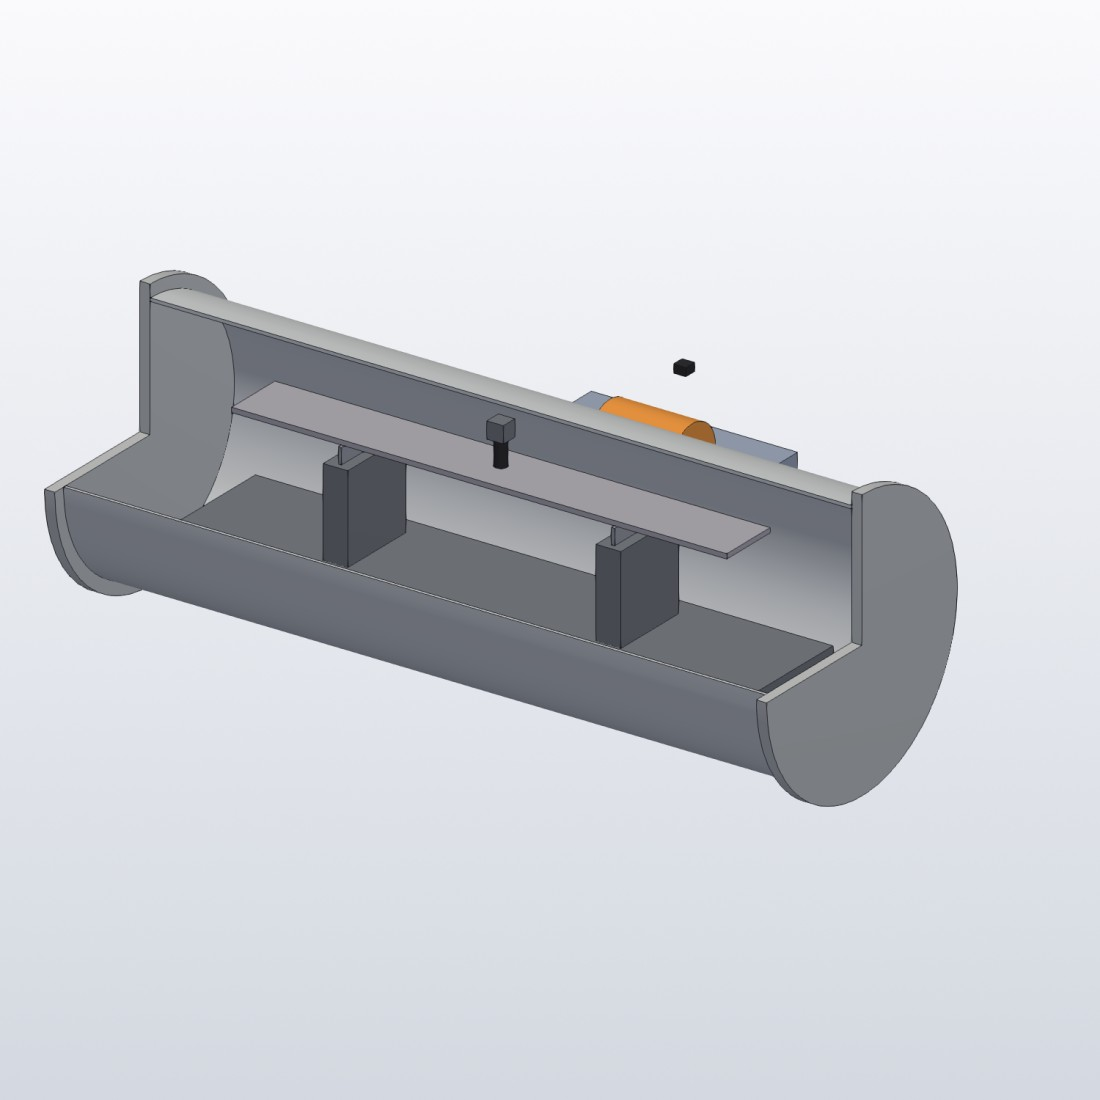
\includegraphics[width=0.34\textwidth]{fig/T4b_detector_cutaway.jpg}
\caption{T4 concepts: (a) nN balance with co-moving grounded cans (cutaway); (b) 42\,Hz resonant detector, Ti-6Al-4V beam $1200\times150\times11.6$\,mm ($f_1=42.0$\,Hz).}
\end{figure}

\testhead{T2\sep Conductor and stator field (B6)}{about \$1.6--3.0M}
\lab{What it decides.} A rotor cooled only by radiation runs at the temperature its field ripple sets. B6 is quench-safe only if the tape's current density at that temperature keeps the current fraction $i\le0.506$, and only if the stator's field is even enough along the rotor's path.
\lab{T2a: conductor.} Thick-film REBCO tape (4\,$\mu$m film, Hf/Zr-doped) on 50\,$\mu$m and 0.1\,mm bases with a thicker copper stabilizer. Measure the critical current at 30\,T at 4.2, 10, 15, 20 and 25\,K in a variable-temperature insert at a 31--45\,T user facility, plus the lengthwise uniformity of 40\,m pieces. Pass: $J_e\ge11.6\un{kA/mm^2}$ at the operating temperature; the 50\,$\mu$m basis is predicted to pass up to about 24.5\,K. Ramp the field at spin-up rates: flux jumps seen at 4.2\,K are predicted to vanish at 15--25\,K (the margin improves 18--50 times); fail if they persist.
\lab{T2b: stator field map.} The allowed azimuthal ripple is about 6--80\,ppm of 30\,T at the first harmonic (0.17--2.3\,mT). Build a REBCO ring coil of at least 1\,m diameter (concept: $4\times250$ turns of 12\,mm tape, 3.2\,km, at 20\,K); map the field on the orbit radius with a rotating search coil or Hall array; correct with shims and trim coils, as superconducting cyclotrons do. Pass: first-harmonic ripple within the target, and drift within it over 24\,h. Fail: no correction below about 100\,ppm. Caution: the one REBCO cyclotron magnet built for field accuracy quenched at 46\,\% of its design current; protect and instrument the ring accordingly.

\begin{figure}[H]
\centering
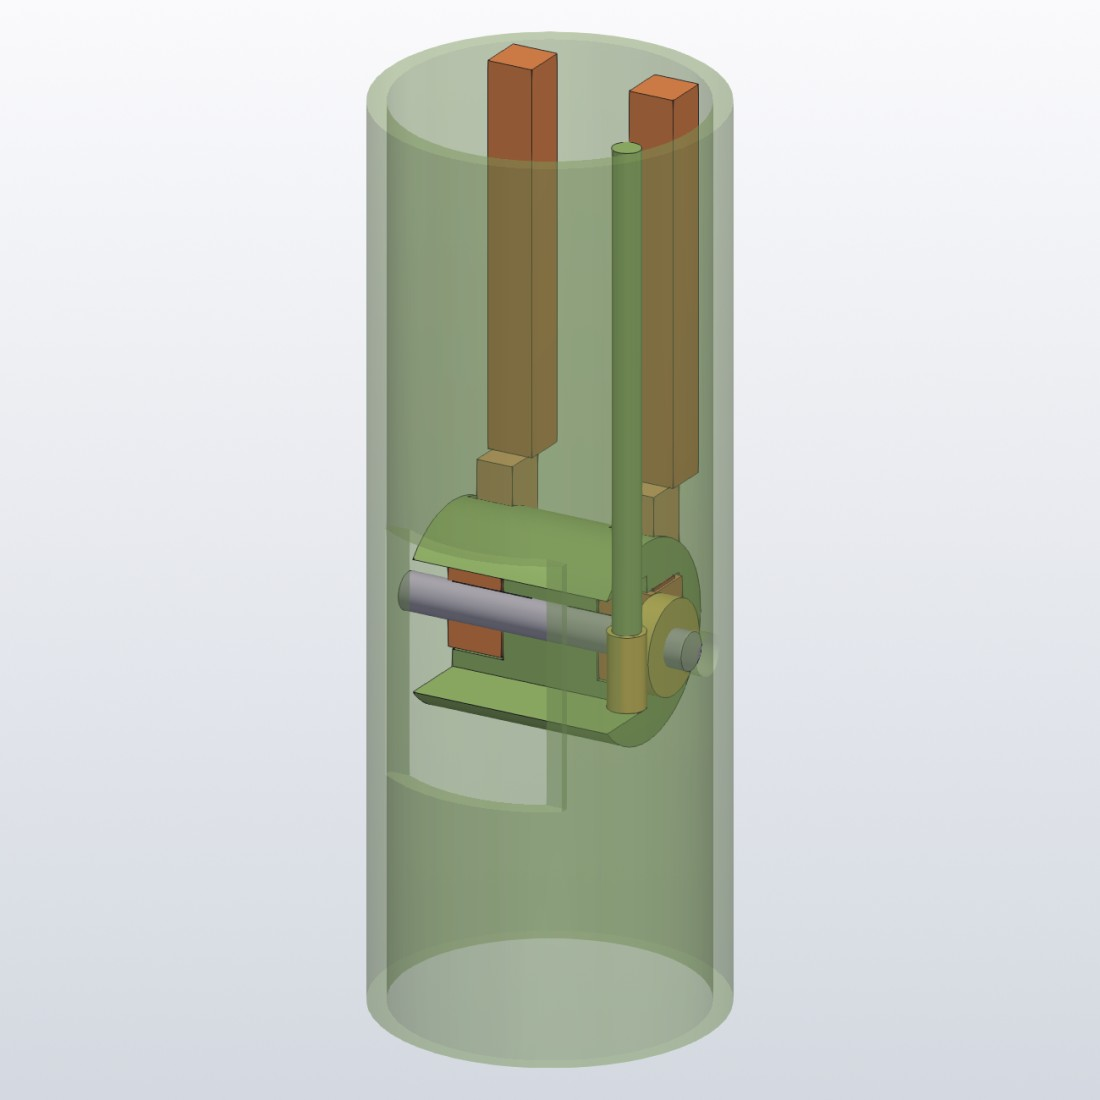
\includegraphics[width=0.22\textwidth]{fig/T2a_head_iso.jpg}\hspace{6mm}
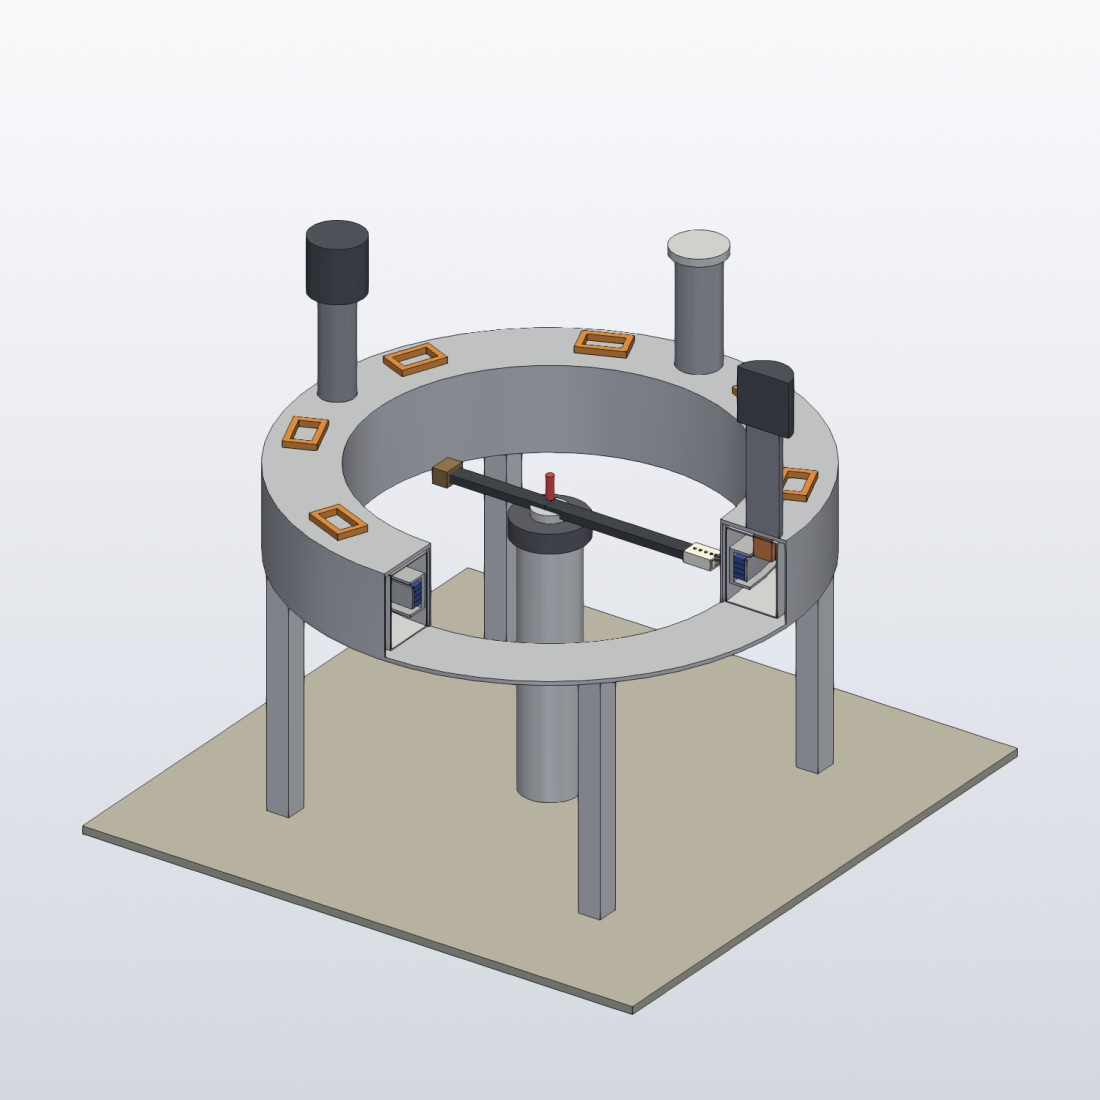
\includegraphics[width=0.40\textwidth]{fig/T2b_ring_cutaway.jpg}
\caption{T2 concepts: (a) variable-temperature probe head for critical-current and flux-jump tests at 30\,T; (b) REBCO ring coil with a rotating field-mapping arm (quadrant cutaway).}
\end{figure}

\testhead{T3\sep A light-driven film inside a laser cavity (B7)}{about \$0.7--1.2M}
\lab{What it decides.} Whether a light-driven, superconducting-like state in \Kc{} can be kept on by re-driving it inside a laser cavity, and whether it is a superconductor at all. Driven \Kc{} shows superconducting-like optics, pressure dependence and nonlinear transport \cite{mitrano}, but a field-expulsion search found none at about 50\,nT ($\chi_v>-0.1$) \cite{devecchi}, and no independent group has reproduced the state.
\lab{Setup.} A 10--20\,nm \Kc{} film grown by molecular-beam epitaxy (12--24 monolayers) on sapphire or diamond, capped against air. Drive at $30\,\mu$m (10\,THz) inside a free-electron-laser cavity such as FELICE at FELIX \cite{felice}: inside the cavity the source pays only for what the film absorbs, and lasing needs the film's absorption (0.1--0.2) below the cavity's headroom. FELICE's fluence at focus is 81--133 times the hold fluence, so the film can sit 0.6--0.7\,m off focus; its 1\,GHz micropulse trains re-drive the film about 8,000 times per macropulse. A cryogenic film station is new hardware.
\lab{Measurements and controls.} Through the macropulse: infrared reflectivity, on-chip transport and Faraday-rotation magnetometry at 50\,nT or better. Controls: off-resonance drive, fluence below threshold, an undoped C$_{60}$ film, base temperatures from below $T_c$ to 300\,K, and the cavity without a film.
\lab{Pass or fail.} Pass: zero resistance and field expulsion held through the macropulse at 100\,K or above, a sustained light-driven superconductor. Fail: no expulsion at the resolution; the state is not superconducting and the path closes. Design check from the drawings: at Brewster incidence the film plane receives only 0.39 of the beam fluence, and each macropulse heats the film column from 100\,K to about 155--180\,K, so the station includes an on-chip thermometer and a shorter-macropulse fallback.

\begin{figure}[H]
\centering
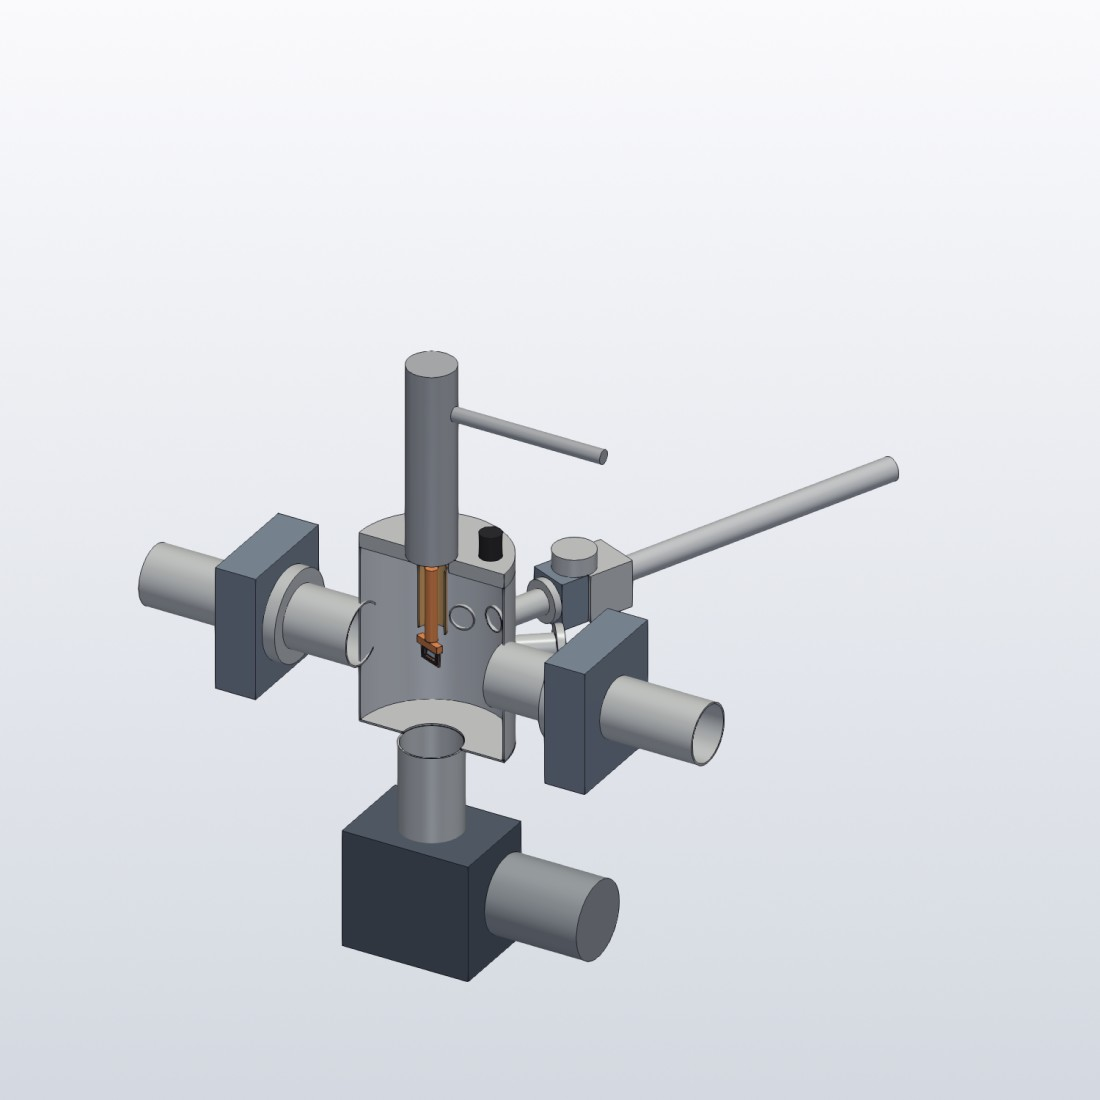
\includegraphics[width=0.34\textwidth]{fig/T3_station_cutaway.jpg}\hspace{4mm}
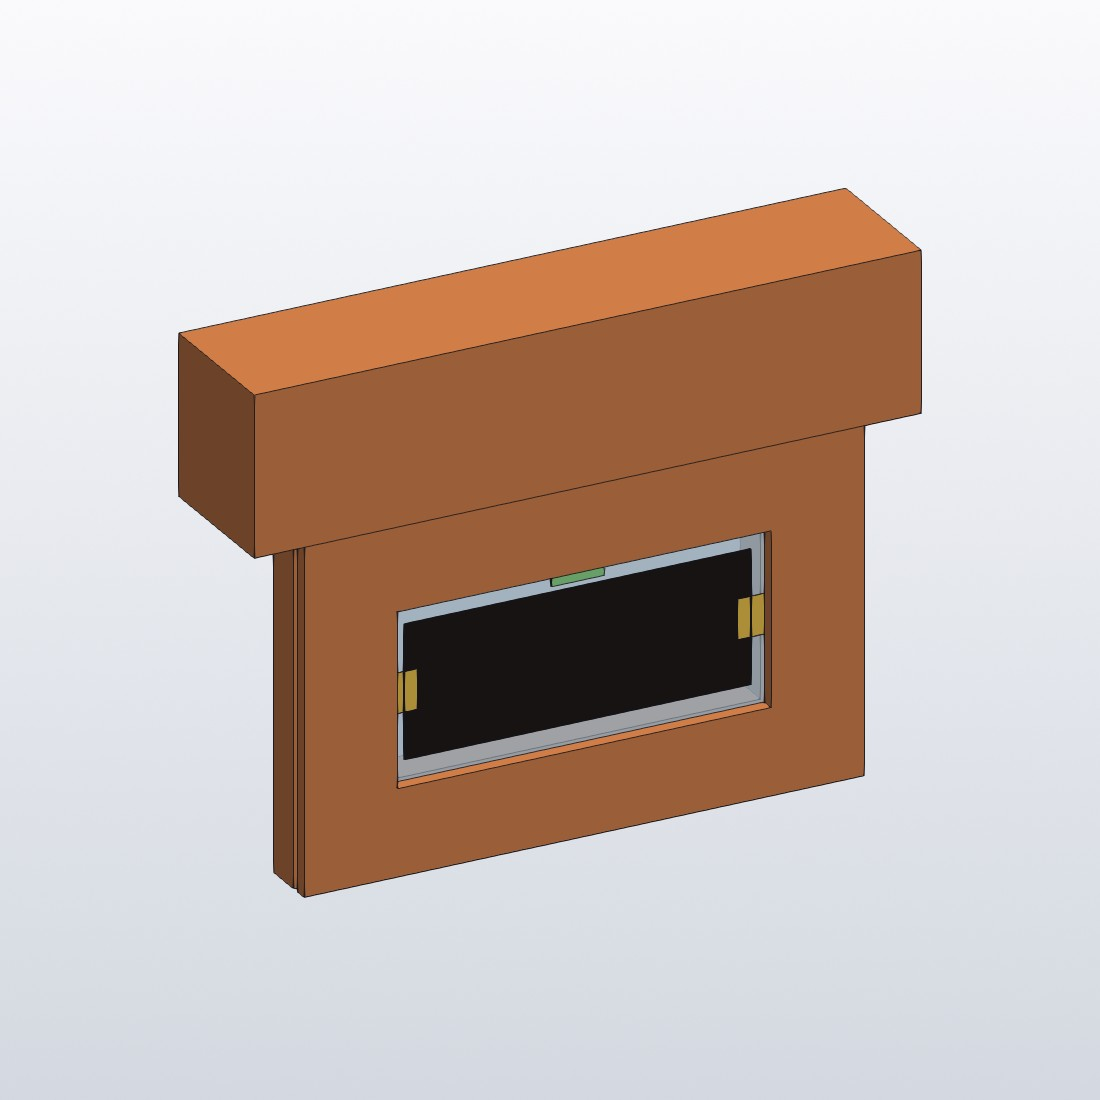
\includegraphics[width=0.28\textwidth]{fig/T3_holder_iso.jpg}
\caption{T3 concepts: (a) cryogenic film station in the laser cavity (cutaway); (b) film holder behind a diamond Brewster plate.}
\end{figure}

\testhead{T1\sep Tangential coupon shot (B6 containment)}{about \$1.1--2.6M}
\lab{What it decides.} The loop proved that debris sliding on a wall loads it exactly as the held rotor loaded its stator, $\lambda v^2/R$, so a containment needs no more tension than the rotor it held. If that holds in practice, the stator itself can be the containment and the craft is 1.3--2.3 times its 312\,kg minimum. If not, containment is far heavier.
\lab{Why a small shot is a full test.} A coupon cut from the rotor's section, sliding on a track of the rotor's radius, presses with the craft's own wall pressure, $\lambda v^2/(Rh)$, whatever its size. Its exit speed after an arc $\theta$ is $v\,e^{-\mu\theta}$, so one shot also measures the friction that sets how fast debris slows.
\lab{Setup.} An 8.9\,g coupon of the real tape stack ($20\times25\times2.2$\,mm), flown along its length in a separating sabot from a two-stage light-gas gun with a 38\,mm launch tube \cite{swri}, onto a concave track of 2.0\,m radius and 30--90$^\circ$ of arc, entering tangentially at a gap of 1, 5 or 20\,mm. Shot matrix: 3.0\,km/s (80\,MPa on the wall) and 6.28\,km/s (351\,MPa, the craft's own), three gaps, two wall materials, repeated.
\lab{Measurements.} Entry and exit speed by photonic Doppler velocimetry ($\mu=-\ln(v_{\rm out}/v_{\rm in})/\theta$, resolved to $\pm0.027$ over $30^\circ$ with 1\,\% velocimetry); back-face strain gauges along the arc; coupon attitude by flash X-ray; high-speed imaging through polycarbonate witness plates; gouges and erosion afterwards.
\lab{Pass or fail.} Pass if the line load follows $\lambda v^2/R$ within about 20\,\% after the entry impact and erosion stays within the ablator budget. Fail if the load stays well above it, if debris escapes inward with more than its share of energy, or if gouging cuts through the ablator. Gouging is expected: 6.28\,km/s is 1.6--4.2 times above known rail and barrel gouging thresholds.

\begin{figure}[H]
\centering
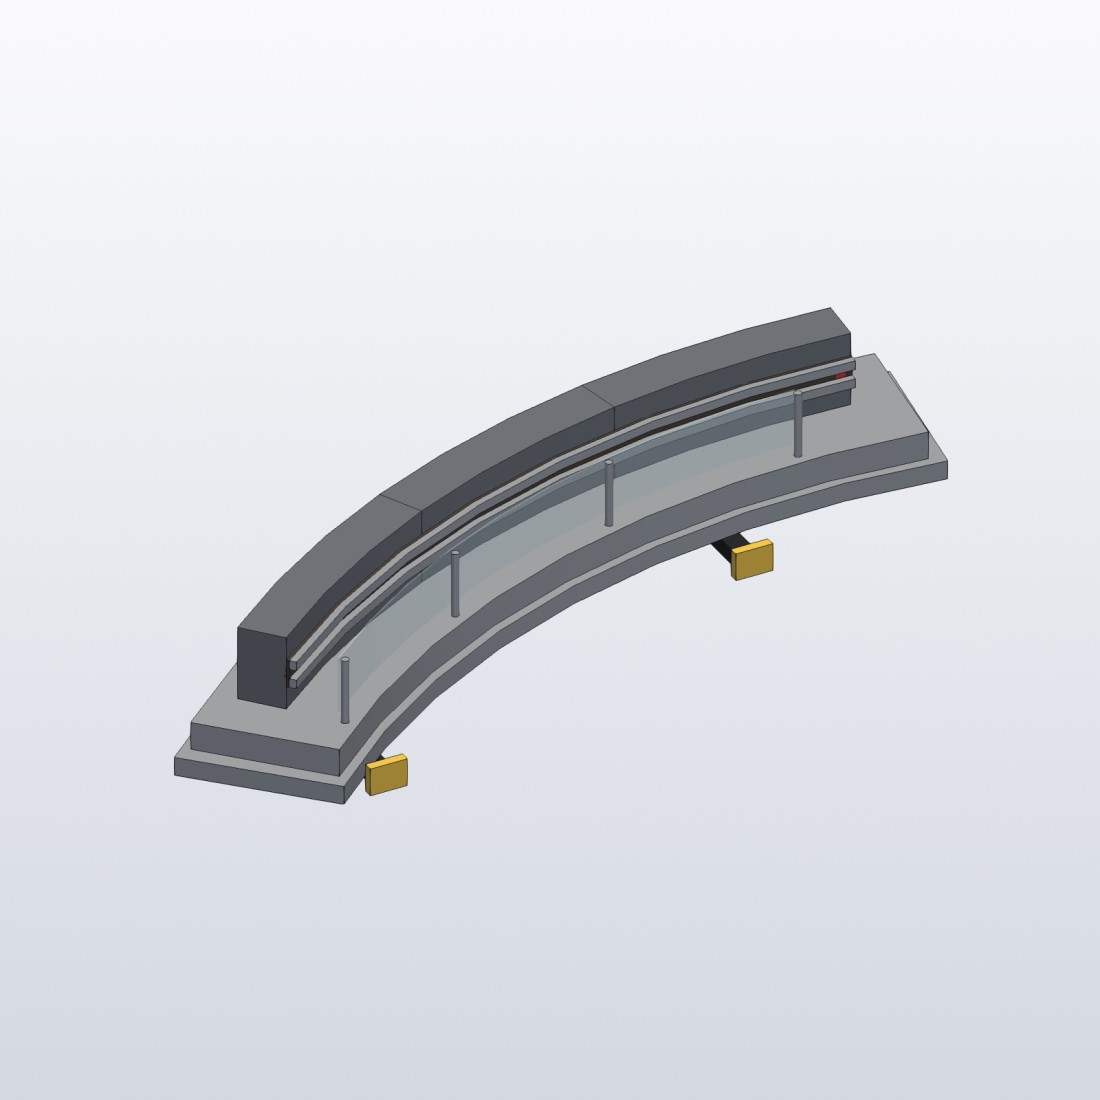
\includegraphics[width=0.40\textwidth]{fig/T1_fixture_iso.jpg}\hspace{4mm}
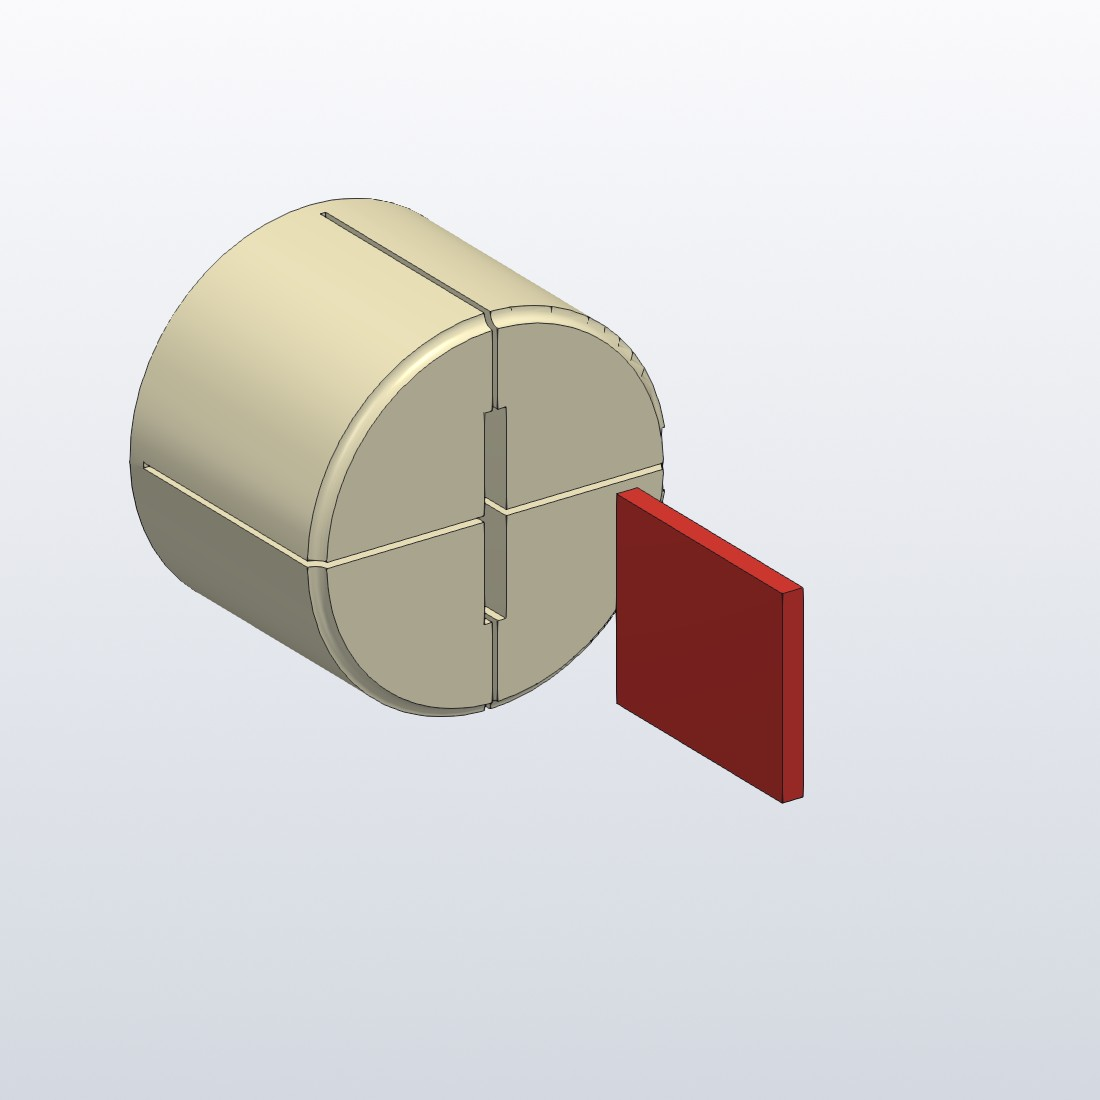
\includegraphics[width=0.26\textwidth]{fig/T1_coupon_sabot_exploded.jpg}
\caption{T1 concepts: (a) the R\,2000 curved track fixture (668\,kg); (b) the coupon (red) and its four-petal sabot.}
\end{figure}

\section{Programme and costs}
Costs are rough order of magnitude ($\pm50\,\%$, US dollars), assuming that magnet and laser time is won by peer-reviewed proposal at no charge, and staff at about \$150--250k per full-time year. The National MagLab gives magnet time free of charge through a competitive proposal process \cite{maglab}; FELIX beam time is also by proposal, with deadlines on 15 May and 15 November \cite{felix}.

\begin{center}\small
\arrayrulecolor{ink}
\begin{tabularx}{\textwidth}{@{}l l r X@{}}
\toprule
\textbf{Test} & \textbf{Facility} & \textbf{ROM cost} & \textbf{Main cost drivers}\\
\midrule
T5 X1 charge control & vacuum lab with a torsion balance & \$0.2--0.5M & balance, sealed box, UV/e-flood, staff; much less at a partner lab with an existing balance\\
T4 field--gravity null & vacuum lab; resonant detector & \$0.7--1.3M & nN balance, resonant beam detector, shielding, staff\\
T2 conductor and stator & 31--45\,T user facility; ring lab & \$1.6--3.0M & 3.2\,km of 12\,mm REBCO, 20\,K cryocooler, mapping arm, quench protection\\
T3 film in an FEL cavity & FEL user facility; MBE lab & \$0.7--1.2M & films, cryogenic intracavity station, diagnostics\\
T1 coupon shot & light-gas-gun range & \$1.1--2.6M & range time, track fixture, velocimetry, high-speed cameras\\
\midrule
\textbf{All five} & & \textbf{\$4--9M} & about 3 years\\
\textbf{First answers (T5 + T4)} & & \textbf{\$1--2M} & \\
\bottomrule
\end{tabularx}
\end{center}
A sensible first step is T5 at a laboratory that already runs a vacuum thrust balance; such balances resolve 100\,nN for test articles of up to 10\,kg \cite{tajmar18}.

\section{What each result would mean}
\begin{center}\small
\begin{tabularx}{\textwidth}{@{}l X X@{}}
\toprule
\textbf{Test} & \textbf{If the expected (null or failing) result} & \textbf{If the opposite}\\
\midrule
T5 & The force dies with the charge: static electricity; the X1 claim is closed. & A force survives a sealed, grounded box in vacuum: outside laboratories must replicate it.\\
T4 & A null, as theory predicts: the inertial-mass-reduction premise closes on data. & A signal that survives every check: new physics.\\
T2 & The ring quenches or cannot be corrected: B6 needs a colder, heavier design or goes back to paper. & It holds at 20\,K: the rotor's magnets can work at their own radiative temperature.\\
T3 & No field expulsion: the driven state is not a superconductor; the B7 path closes. & Zero resistance and expulsion held on: a new, light-powered route to superconductivity.\\
T1 & Debris presses harder than the rotor did: containment gets far heavier. & Debris presses no harder: the stator itself is the containment and the craft stays light.\\
\bottomrule
\end{tabularx}
\end{center}
A null is still an answer: each of these tests ends an argument with data, whichever way it falls, and every result feeds the next loop.

\section{What would restart the loop}
Re-checks from February 2027 (a new ambient-pressure superconducting record above 151\,K or a pressure-quenched hydride; nonlinear Breit--Wheeler pair production at SLAC E-320); an outside test or paper on the X1 claim; an independent reproduction of driven \Kc; a field map of a large REBCO ring, or a REBCO cyclotron reaching its design field; and any result from T1--T5.

\section{Limitations}
\begin{itemize}
\item The rigs are concept designs for review, not for manufacture; facility items (guns, magnets, lasers) are drawn indicatively.
\item Costs are rough order of magnitude, $\pm50\,\%$.
\item The renders and the film show simulated concept rigs; only the T2 field lines are computed physics (Biot--Savart).
\item The X1 and driven-\Kc{} claims belong to others and are described from public sources; T5 needs access to an X1 device.
\item This is AI-assisted work (Section~2). Every number can be checked against the code and sources in the supplements; please report errors.
\end{itemize}

\section{Contents of this record}
\begin{itemize}
\item \textbf{This report} (PDF).
\item \textbf{S1} Mathematics run sheet, run 11 (final), 40 pages: every derivation with its inputs, proofs and references.
\item \textbf{S2} A3 drawing set PTP-000 to PTP-902 (20 sheets): general arrangements, sections, schematics, block diagrams and equipment lists for T1--T5.
\item \textbf{S3} CAD package: 8 STEP assemblies, DXF views, renders, drawing and model scripts, computed numbers, equipment list.
\item \textbf{S4} Research sheets: 40 illustrated sheets (numbered CT-11 to CT-67), grouped by the test each one feeds, with a contents page, in the author's dark sheet style. The loop's own health checks and run summaries are left out; their data is in S5.
\item \textbf{S5} Loop records and code: the final state file, test plans, costs, prompts, search logs (162 searches with sources), and the Python that computes and cross-checks every number.
\item \textbf{S6} Film, 1:52, ``PAIS GAP LOOP $\cdot$ Test Programme'' (simulated concept rigs, with soundtrack; the music is not covered by this record's licence: all rights reserved by its rights holder).
\end{itemize}

\section*{How to cite}
\AUTHOR\ (2026). \emph{Five Experiments to Settle What Is Left of the Pais Patents: open designs, costs and what each result would mean.} Version 1.0. Zenodo. DOI as shown on the record.

\begin{thebibliography}{99}\small
\setlength{\itemsep}{1pt}
\bibitem{p532} S.\,C. Pais, ``Craft using an inertial mass reduction device'', US Patent 10,144,532 B2 (2018).
\bibitem{p366} S.\,C. Pais, ``Electromagnetic field generator and method to generate an electromagnetic field'', US Patent 10,135,366 B2 (2018).
\bibitem{p827} S.\,C. Pais, ``High frequency gravitational wave generator'', US Patent 10,322,827 B2 (2019).
\bibitem{p733} S.\,C. Pais, ``Plasma compression fusion device'', US 2019/0295733 A1 (2019).
\bibitem{p597} S.\,C. Pais, ``Piezoelectricity-induced room temperature superconductor'', US 2019/0348597 A1 (2019).
\bibitem{exodus} Exodus Propulsion Technologies, ``System and method for generating forces using asymmetrical electrostatic pressure'', US Patent 11,511,891; company presentation and press reports (claims; no independent test as of November 2026).
\bibitem{mitrano} M. Mitrano \emph{et al.}, ``Possible light-induced superconductivity in K$_3$C$_{60}$ at high temperature'', Nature \textbf{530}, 461 (2016).
\bibitem{devecchi} G. de Vecchi \emph{et al.}, ``Upper limit on magnetic field expulsion in optically driven K$_3$C$_{60}$'', Phys.\ Rev.\ Research \textbf{7}, 043270 (2025).
\bibitem{hathaway} G. Hathaway, L.\,L. Williams, ``Null-result test for effect on weight from large electrostatic charge'', Physics \textbf{3}, 160 (2021).
\bibitem{tajmar21} M. Tajmar \emph{et al.}, ``High-accuracy thrust measurements of the EMDrive and elimination of false-positive effects'', TU Dresden (2021).
\bibitem{tajmar18} M. Tajmar \emph{et al.}, ``SpaceDrive: thrust balance development and first measurements of Mach-effect and EMDrive thrusters'', IAC-18-C4.7-C3.5.5 (2018).
\bibitem{tajmar24} M. Tajmar, M. K\"o{\ss}ling, O. Neunzig, ``In-depth experimental search for a coupling between gravity and electromagnetism with steady fields'', Sci.\ Rep.\ \textbf{14} (2024).
\bibitem{brack22} T. Brack \emph{et al.}, ``Dynamic measurement of gravitational coupling between resonating beams in the hertz regime'', Nat.\ Phys.\ \textbf{18}, 952 (2022).
\bibitem{felice} B.\,L. Militsyn \emph{et al.}, ``FELICE: the free electron laser for intra-cavity experiments'', Nucl.\ Instrum.\ Methods A (2003).
\bibitem{swri} Southwest Research Institute, ``Large two-stage light-gas gun facility'' (38\,mm launch tube, 7\,km/s).
\bibitem{maglab} National High Magnetic Field Laboratory, ``Requesting magnet time'', \url{https://nationalmaglab.org/user-resources/requesting-magnet-time/}.
\bibitem{felix} FELIX Laboratory, ``Use our facility: apply for beam time'', \url{https://www.ru.nl/felix/facility/}.
\bibitem{hl3} Organization for Ethical Source, ``Hippocratic License 3.0'', \url{https://firstdonoharm.dev}.
\end{thebibliography}
\noindent{\small Further references for every item are in Supplement S1 and the search logs in S5.}
\end{document}
